\documentclass[aspectratio=43]{beamer}

\usepackage[utf8]{inputenc}
\usepackage{svg}
\usepackage{xcolor}
\usetheme{lmu}

\title{Superresolution}
\author{B.Schüss, I. Frumin, L. Obermeier, S. Gavra, Y. Chen}
\subtitle{Saving caribous by counting trees}
\institute[DBS]{Team4 - Praktikum Big Data Science}


\begin{document}

\begin{frame}[plain]
\titlepage
\end{frame}

\section{Section A}

\subsection{Subsection 1}

\subsubsection{Subsubsection i}

\begin{frame}{Motivation}

	\begin{figure}[h]	
		\minipage{0.32\textwidth}
		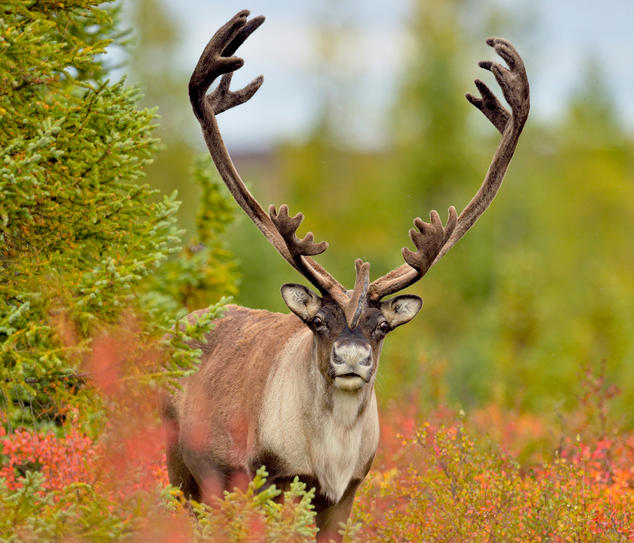
\includegraphics[width=\linewidth , height=110]{img/caribou.jpg}
		\caption{Caribous}
		\endminipage\hfill
		\minipage{0.32\textwidth}
		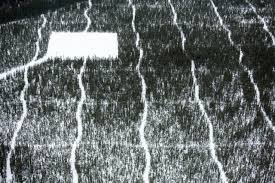
\includegraphics[width=\linewidth , height=110]{img/seismic_lines.jpg}
		\caption{The Problem}
		\endminipage\hfill
		\minipage{0.32\textwidth}
		
\includegraphics[width=\linewidth , height=110]{img/smart_wolves.jpeg}
		\caption{Smart wolves}
		\endminipage\hfill
	\end{figure}
\end{frame}

\begin{frame}{The Datasets}
	\bigskip\bigskip\bigskip\bigskip\bigskip\bigskip
	\minipage{0.40\textwidth}
		
	\begin{block}{5m (1px=3.5mm)}
	\begin{itemize}
		\item Slices of 512x512 
		\item winter \& summer
		\item seedlings with bounding boxes
		\item overlap
	
	\end{itemize}		
	\end{block}
	
		\begin{block}{30m (1px=7.5mm)}
	\begin{itemize}
		\item Slices of 256x256
		\item only summer
		\item seedlings with bboxes
	\end{itemize}		
	\end{block}
	\endminipage\hfill
	\minipage{0.59\textwidth}
		\begin{figure}
			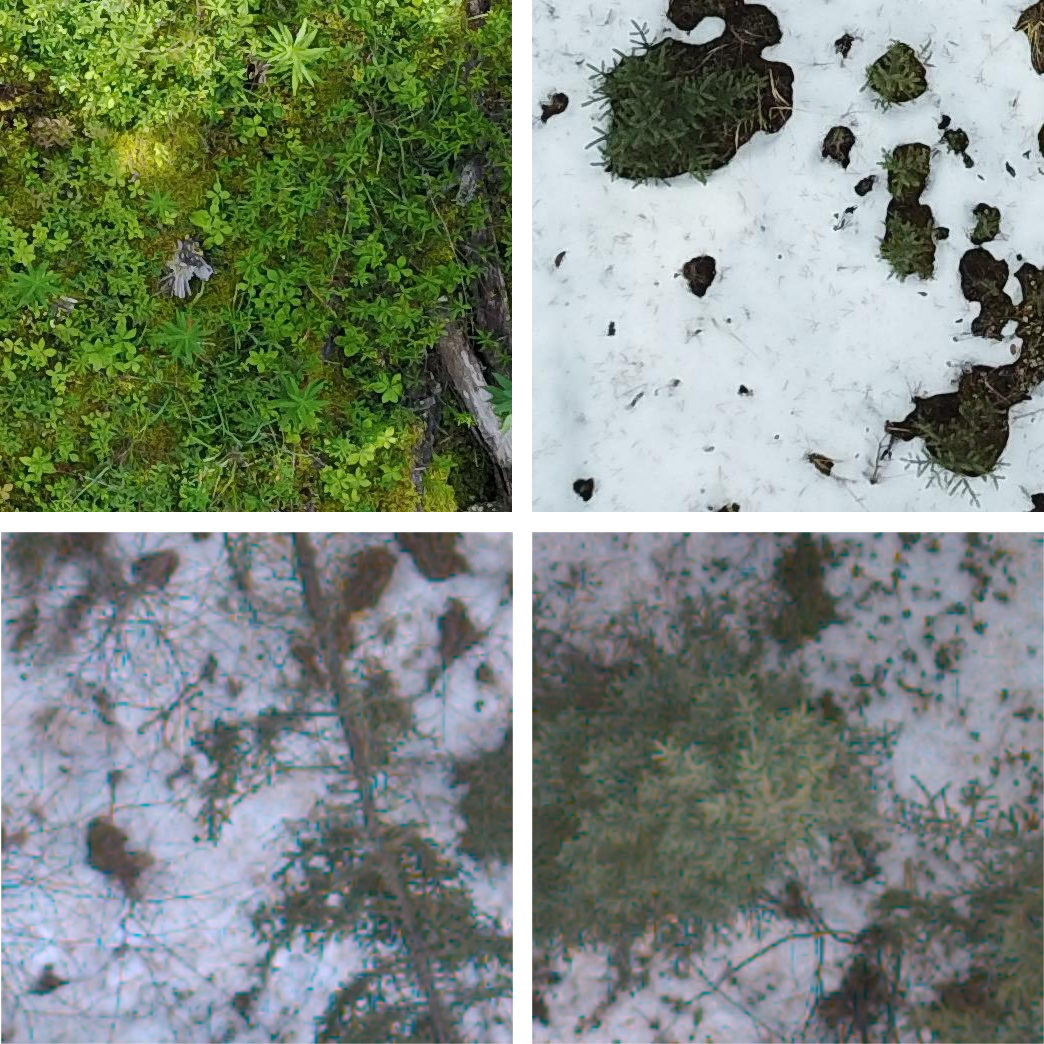
\includegraphics[height= 160]{img/dataset.png}
			
		\end{figure}	

	\endminipage\hfill
\end{frame}

\begin{frame}{Superresolution- Approaches}
	\bigskip\bigskip
	\begin{block}{5m images \rightarrow  gauss blur (radius=2) \rightarrow resize}
	\begin{itemize}
		\item Bicubic Interpolation
		\item SRCNN $\rightarrow$ 3 conv layers
		\item SRGAN $\rightarrow$ residual blocks + up-sampling block, G vs. D
		\item SFTGAN $\rightarrow$ priors, segmentation maps, G vs. D
	\end{itemize}
	\end{block}
	
	\begin{exampleblock}{Data augmentation}
	\begin{itemize}
		\item SRCNN $\rightarrow$ random rotation, \& flipping
		\item SRGAN $\rightarrow$ random cropping
		\item SFTGAN $\rightarrow$ random copping, rotation, \& flipping
	\end{itemize}
	\end{exampleblock}	

\end{frame}


\begin{frame}{Superresolution - 5m results}
	\centering
	\bigskip\bigskip
	\begin{figure}	
		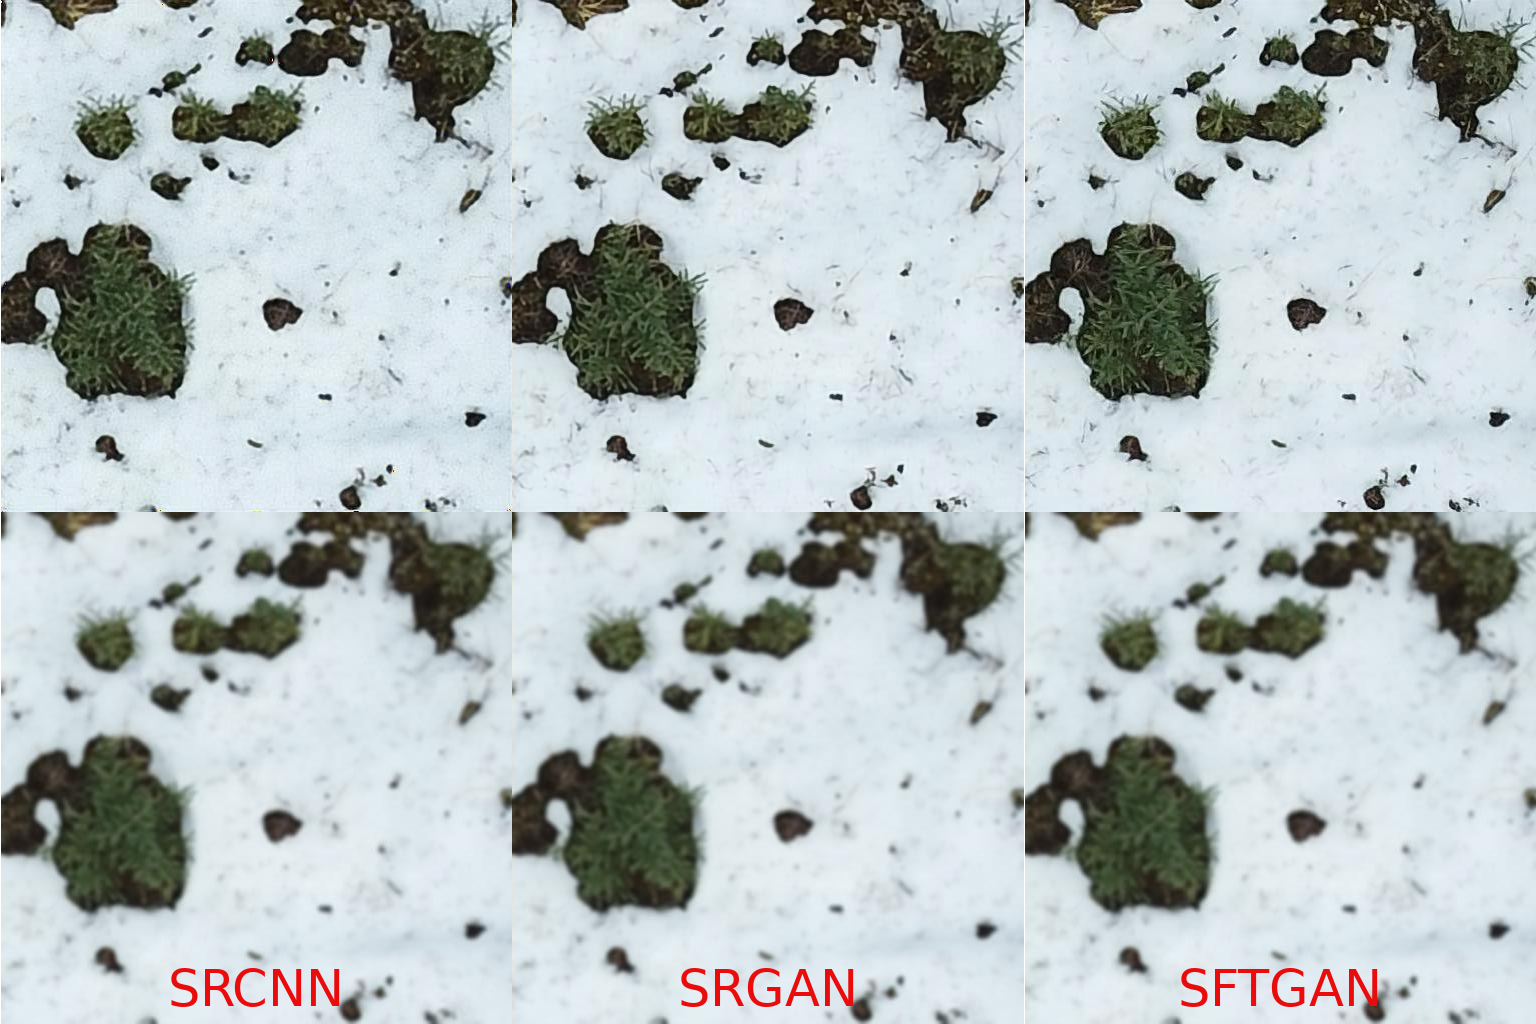
\includegraphics[width=\textwidth]{img/sr-result-5m.png}
	\end{figure}
\end{frame}

\begin{frame}{Superresolution -30m results}
	\centering
	\bigskip\bigskip
	\begin{figure}	
		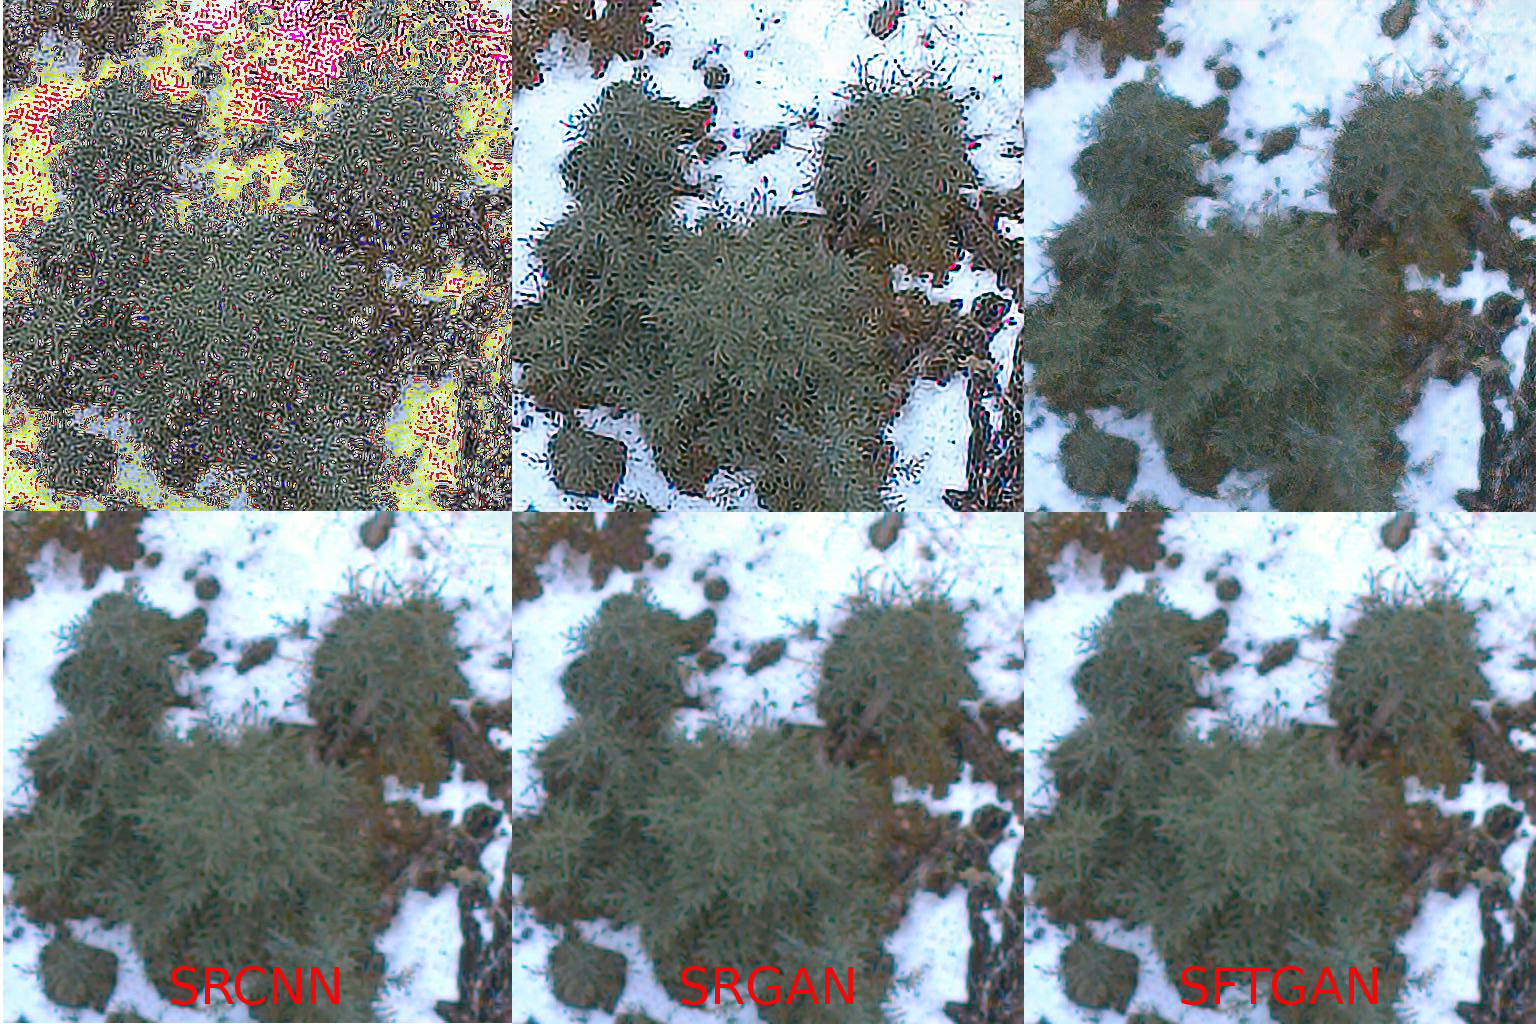
\includegraphics[width=\textwidth]{img/sr-result-30m.png}
	\end{figure}
\end{frame}



\begin{frame}{Object detection}
	\begin{block}{Training}
	\begin{itemize}
		\item 5m images $\rightarrow$ down-sampling $\rightarrow$ SR 
		\item Train object detection on reconstructed images
	\end{itemize}
	\end{block}
	
	\begin{block}{Evaluation for each SRM}
	\begin{itemize}
		\item reconstructed 5m images
		\item superresoluted 30m images
	\end{itemize}
	
	\end{block}
	
\end{frame}

\begin{frame}{Object detection - Results}
	\bigskip\bigskip
	\minipage{0.49\textwidth}
	\begin{block}{5m mAP@.50IoU}
		\begin{itemize}
		\item {\color{red}0.8757 SRGAN}
		\item {\color{blue}0.8697 SRCNN}
		\item {\color{cyan}0.8637 BICUBIC}
		\item {\color{green}0.8481 SFTGAN}
	\end{itemize}		
	\end{block}

	\endminipage\hfill
	\minipage{0.49\textwidth}
	\begin{figure}
		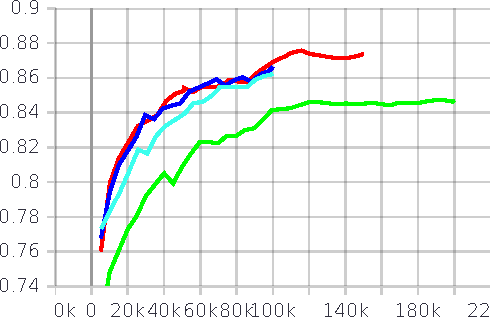
\includegraphics[ height=90]{img/5m_mAP@50IOU.pdf}
		%\includesvg{img/5m_mAP@50IOU}
	
	\end{figure}
	\endminipage\hfill
		\minipage{0.49\textwidth}
	\begin{block}{30m mAP@.50IoU}
	\begin{itemize}
		\item {\color{green}0.4359 SFTGAN}
		\item {\color{cyan}0.4245 BICUBIC}
		\item {\color{gray}0.4060 RAW}
		\item {\color{red}0.2742 SRGAN}
		\item {\color{blue}0.0404 SRCNN}
	\end{itemize}
	\end{block}
		
	
	\endminipage\hfill
	\minipage{0.49\textwidth}
	\begin{figure}
		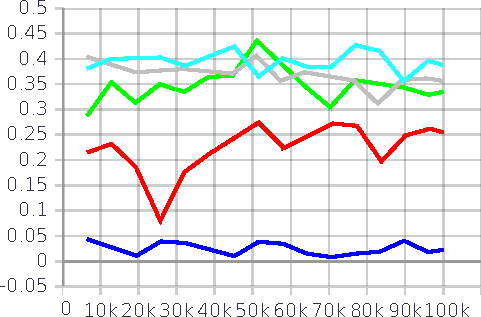
\includegraphics[ height=90]{img/30m_mAP@50IOU.pdf}
	\end{figure}
	\endminipage\hfill

\end{frame}


\begin{frame}{Object detection}
	\begin{exampleblock}{Failed}
	\begin{itemize}
		\item train object detection on raw 5m images
		\item evaluate on superresoluted 30m images
		
	\end{itemize}
	Failed miserably:
	\begin{itemize}
		\item Object detection model, trained on raw images, learned different features, 
		than the super resolution models generate.		
	\end{itemize}
		
	\end{exampleblock}			

\end{frame}



\begin{frame}{Future Work \& Conclusion}
	\begin{block}{Future Work}
	\begin{itemize}
		\item Model optimization
		\item Automatic early stopping on 30m images
		\item Train GAN for down-sampling
	\end{itemize}			
	\end{block}
	\begin{block}{Conclusion}
		\textbf{It works and can be useful!}
	
	\end{block}	
	
\end{frame}

\begin{frame}{Thank you!}
	\bigskip\bigskip
	\centering
	We \& the caribous thank you for your attention!
	\begin{figure}
		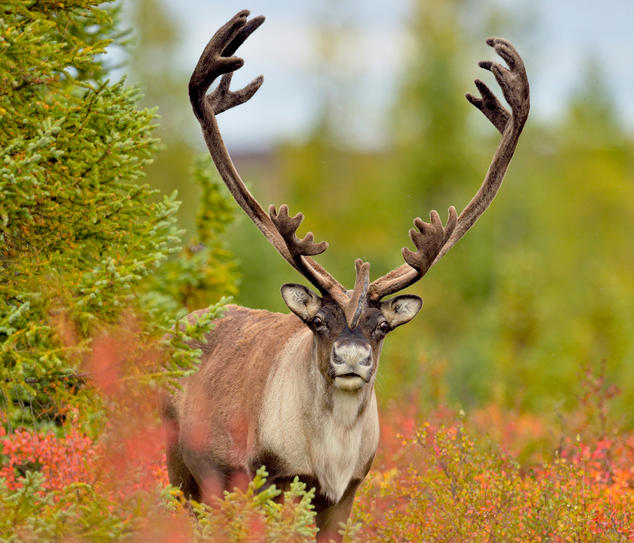
\includegraphics[height=180]{img/caribou.jpg}	
	
	\end{figure}
\end{frame}



\end{document}